\begin{wrapfigure}[23]{r}{.5\textwidth}
  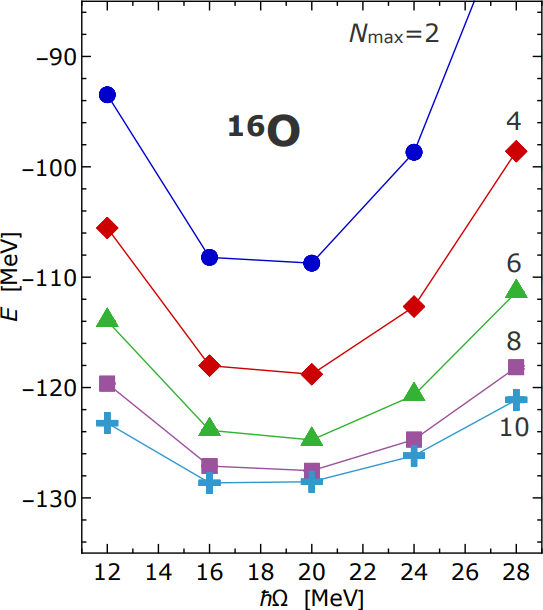
\includegraphics[width=.5\textwidth]{media/freq_filter.png}
  \caption{NCSM calculations for \n{16}{O} in dependency on the used oscillator frequency \cite{sommerschule}.}
  \label{fig:freq_dependency}
\end{wrapfigure}
The single-particle harmonic oscillator basis is not asymptotically good to approximate the states of nuclei, as harmonic oscillator wave functions fall off like a gaussian function, but bound states in a potential well typicall fall off like an exponential function \cite{sommerschule}. Furthermore, the composition into the harmonic oscillator slater determinants is dependant on a free parameter for the oscillator frequency. This oscillator frequency also defines the oscillator length and thus the spatial resolution for the basis states.

As we have already seen, the dependence on the oscillator frequency results in different convergence rates for our NCSM sequences. In fact, NCSM calculations using harmonic oscillator slater determinants typically show a parabolic convergence behaviour with respect to the used oscillator frequency. This is shown in \autoref{fig:freq_dependency} for the nucleus \n{16}{O}. As a consequence, there is a special frequency, for which an optimal convergence rate is to be expected. In \autoref{fig:freq_dependency}, this minimum frequency is given by $\hbar \Omega = \SI{20}{\mega\electronvolt}$.

In order to capture those different convergence rates, we want to restrict the sequences used to either side of the minimum, resulting in two training modes. In the first training mode, only sequences to the left of the frequency minimum are used, such that the network will get trained to modelling the long range behaviour of the nucleonic interaction. Conversely, in the second training mode, the networks will be trained on the short range behaviour by restricting the frequencies to the ones higher than the minimum.

To implement this, we dynamically compute the frequency, for which the lowest value is achieved at $N_\mathrm{max} = 8$ for each NCSM calculation. This frequency will be used to filter the frequencies for the training. In both cases, we include the frequency minimum, as that is the frequency with the best convergence behaviour.



\begin{figure}[H]
  \begin{subfigure}{\textwidth}
    \centering
    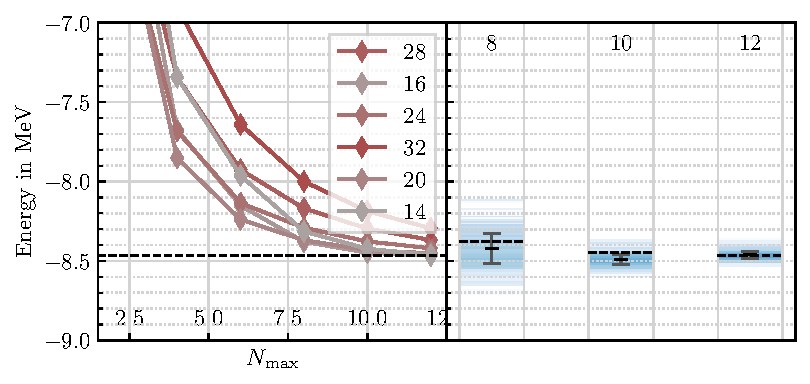
\includegraphics{media/outlook_frequency_lower.pdf}
    \caption{}
  \end{subfigure}
  \begin{subfigure}{\textwidth}
    \centering
    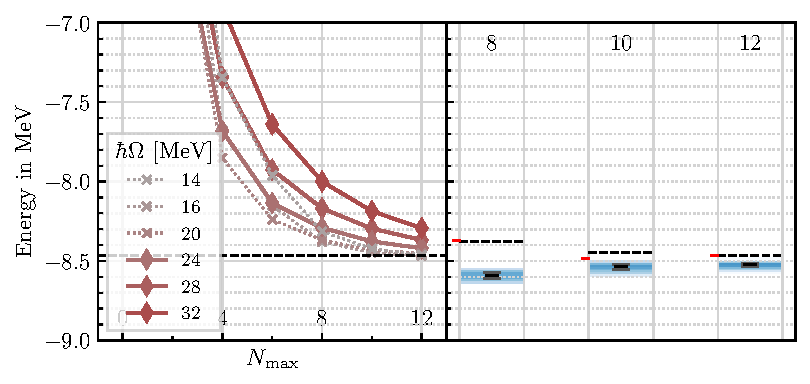
\includegraphics{media/outlook_frequency_higher.pdf}
    \caption{}
  \end{subfigure}
  \caption{Evaluation of the frequency filter training mode on \n{3}{H} with the interaction specified above. In \textbf{(a)}, the networks were trained on the low frequencies, thus modeling the long range behaviour. In \textbf{(b)}, the networks were trained on the high frequencies, thus modeling the short range behaviour.}
  \label{fig:eval_freqfilter}
\end{figure}

We look at a single example of the \n{3}{H} nucleus, using a semi-local momentum space regulated interaction of chiral order 4 with two body interactions and a cutoff at \SI{450}{\mega\electronvolt} alongside a SRG evolution with a flow parameter of \srg{0.08}. Since there are six frequencies available, the evaluation for the long range training mode will include the three lowest and the evaluation for the short range mode will include the three highest frequencies. In \autoref{fig:eval_freqfilter}, the evaluation results are seen for the difference based extrapolation framework.

